\clearpage
\section{Earth}
\subsection{Ground Penetrating Radar}
\subsubsection{Glacial}
\begin{table}[h!]
\centering
\caption{Categorised GPR profile keywords for glacial environments. Geometry, reflectivity and continuity are shown in separate columns.}
\begin{tabular}{|p{5cm}|p{5cm}|p{5cm}|}
\hline
\textbf{Geometry / Structure} & \textbf{Continuity} & \textbf{Amplitude / Reflectivity} \\
\hline
Dipping & Continuous & Varied reflectivity \\
Sub-horizontal & Discontinuous & high reflectivity \\
Horizontal & & Low amplitude \\
Downlap & & high \\
Undulating & & \\
Hummocky & & \\
Chaotic & & \\
Wavy & & \\
Oblique & & \\
Diffraction hyperbola & & \\
Planar & & \\
Subparallel & & \\
Noisy & & \\
\hline
\end{tabular}
\label{tab:glacial-keywords}
\end{table}


\begin{figure}[h!]
    \centering
    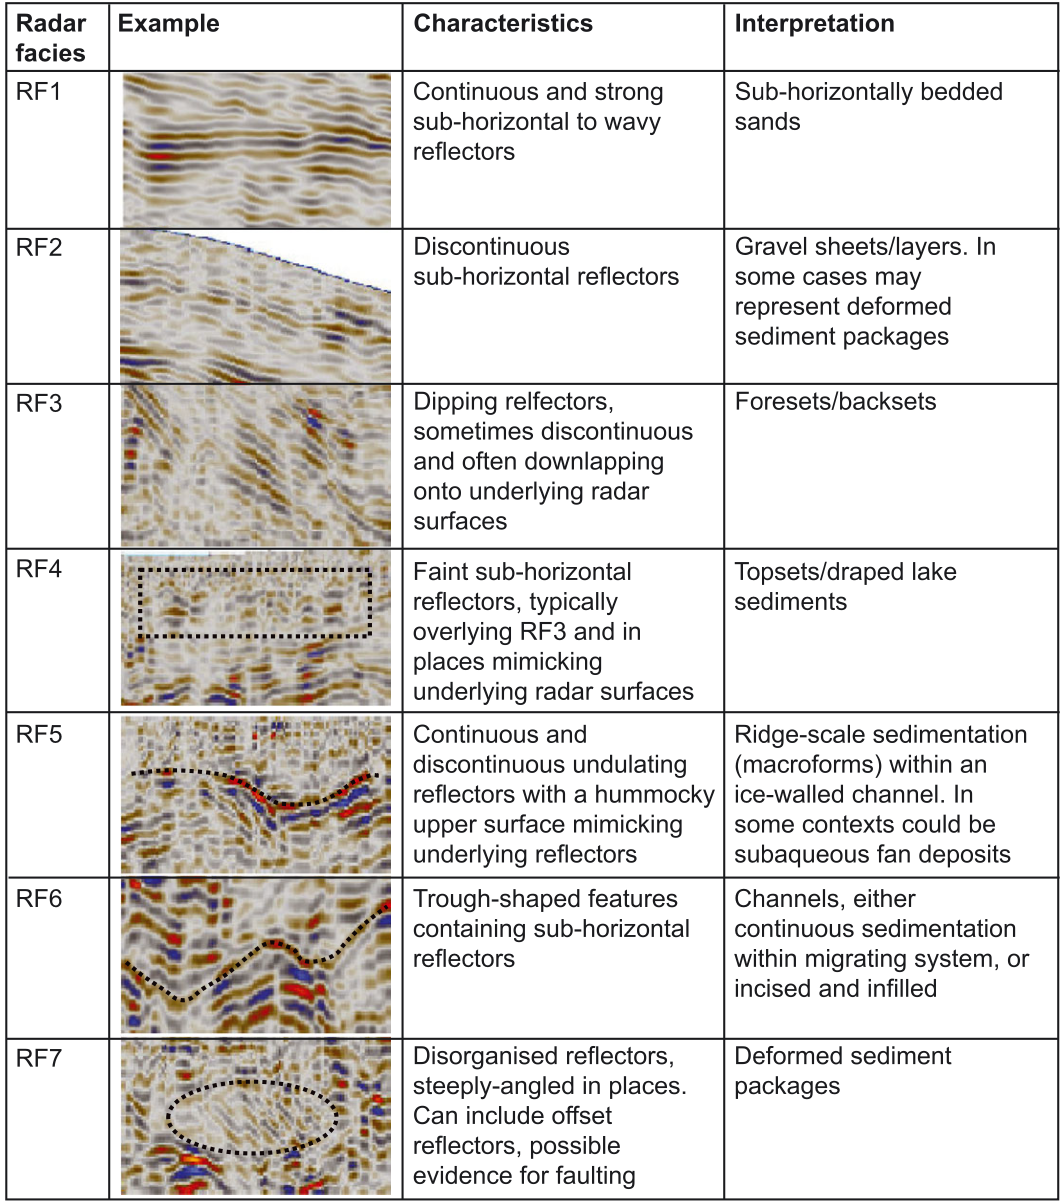
\includegraphics[width=0.9\linewidth]{Figures/0.2GPR/Lovell_2019_1.png}
    \caption[Kame belt morphology (1).]{Kame belt morphology (1). \textbf{Keywords: } Continuous, sub-horizontal, wavy, discontinuous, dipping, downlap, undulating, hummocky, chaotic \citep{Lovell2019}.}
    \label{fig:Lovell2019-1}
\end{figure}
\clearpage
\begin{figure}[h!]
    \centering
    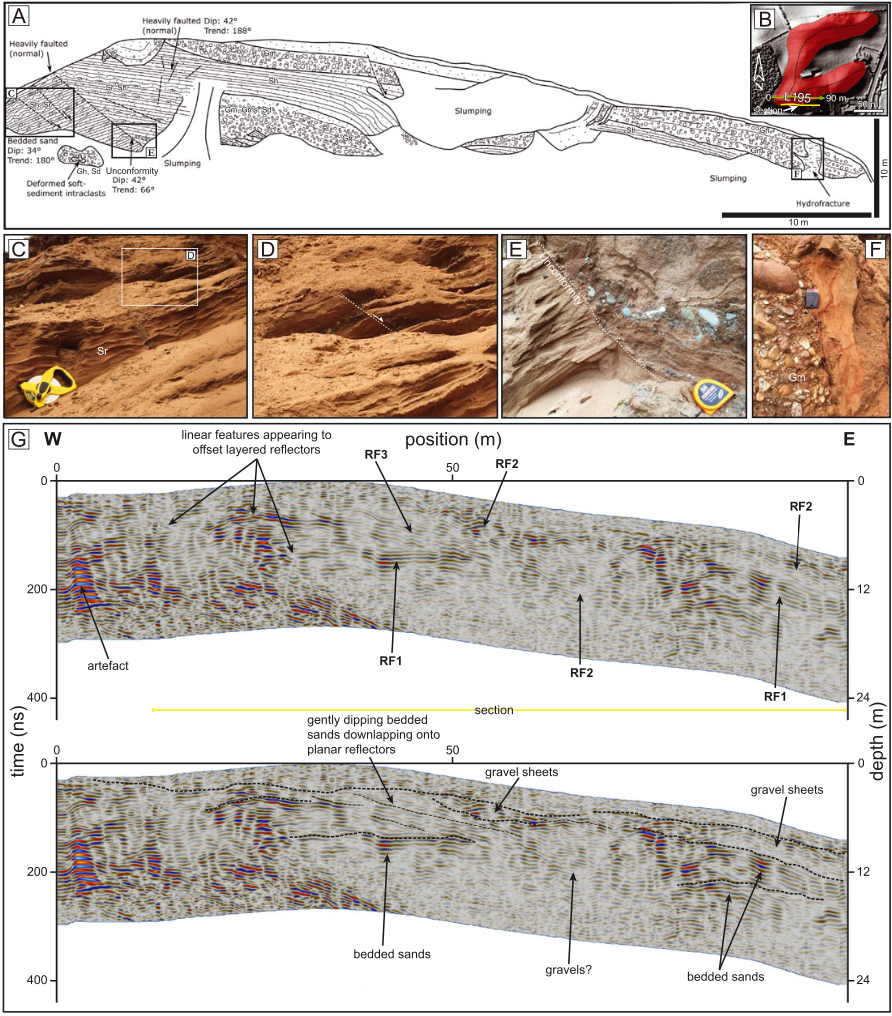
\includegraphics[width=0.9\linewidth]{Figures/0.2GPR/Lovell_2019_3.png}
    \caption[Kame belt morphology (2).]{Kame belt morphology (2). \textbf{Keywords: } Varied reflectivity, discontinuous, downlap, dipping, semi-horizontal \citep{Lovell2019}.}
    \label{fig:Lovell2019-3}
\end{figure}
\clearpage

\begin{figure}[h!]
    \centering
    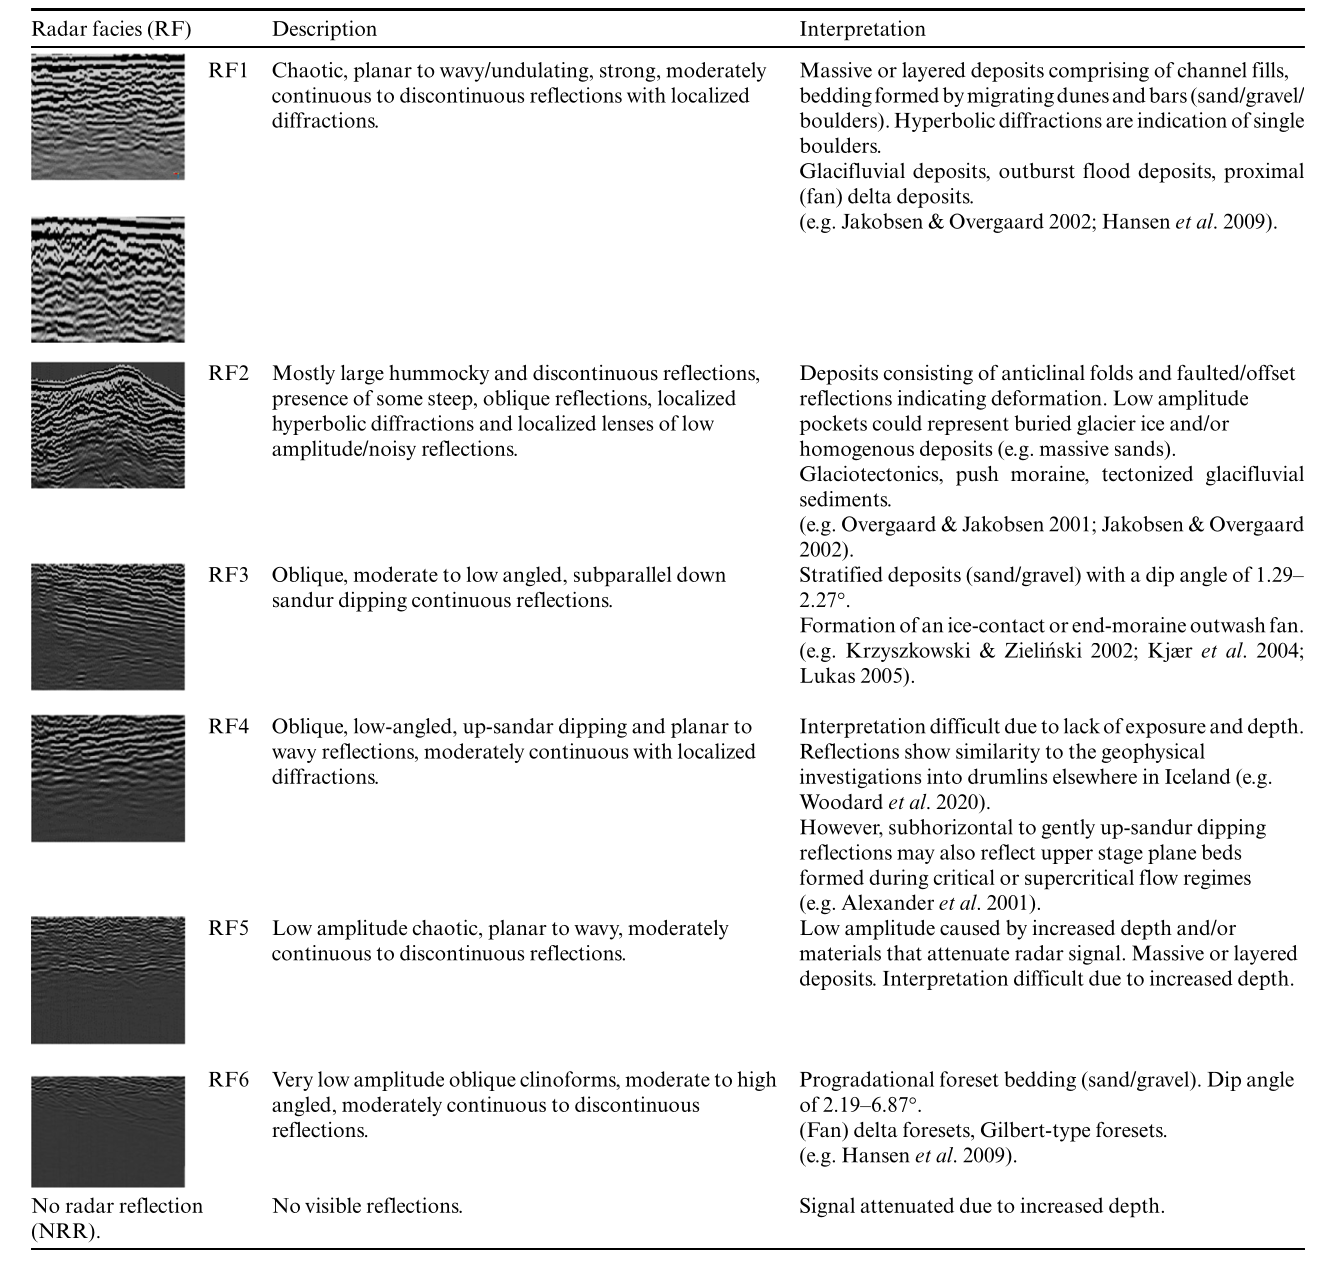
\includegraphics[width=0.9\linewidth]{Figures/0.2GPR/Harrison2022_IceMargin.png}
    \caption[Buried ice-marginal landsystem.]{Buried ice-marginal landsystem. \textbf{Keywords: } Chaotic, planar, wavy, undulating, strong, continuous, discontinuous, diffraction, hummocky, steep, oblique, hyperbolic, noisy, low amplitude, low angled, subparallel, dipping \citep{Harrison2022}.}
    \label{fig:Harrison2022-1}
\end{figure}


\begin{figure}[h!]
    \centering
    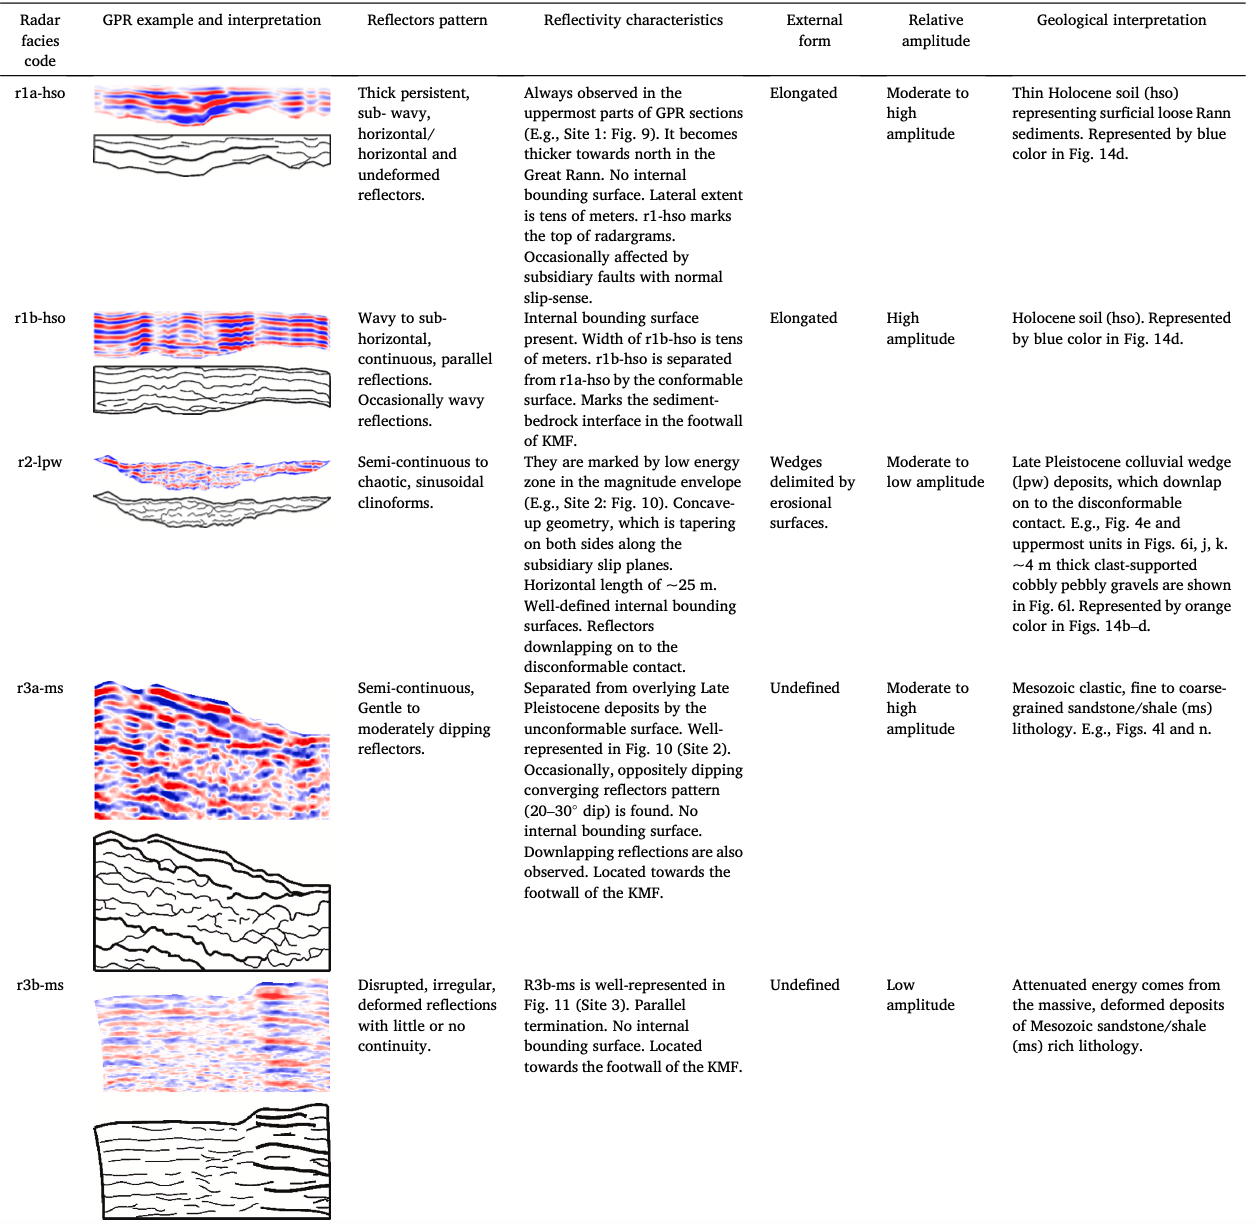
\includegraphics[width=0.9\linewidth]{Figures/0.2GPR/Shaikh2022_fault_1.png}
    \caption[Active fault zone deposits.]{Active fault zone deposits. \textbf{Keywords: } Disrupted, irregular, deformed, low continuity, parallel, low amplitude, semi-continuous, dipping, moderate amplitude, high amplitude \citep{Shaikh2022}.}
    \label{fig:Shaikh2022-1}
\end{figure}

\begin{landscape}
\begin{figure}[h!]
    \centering
    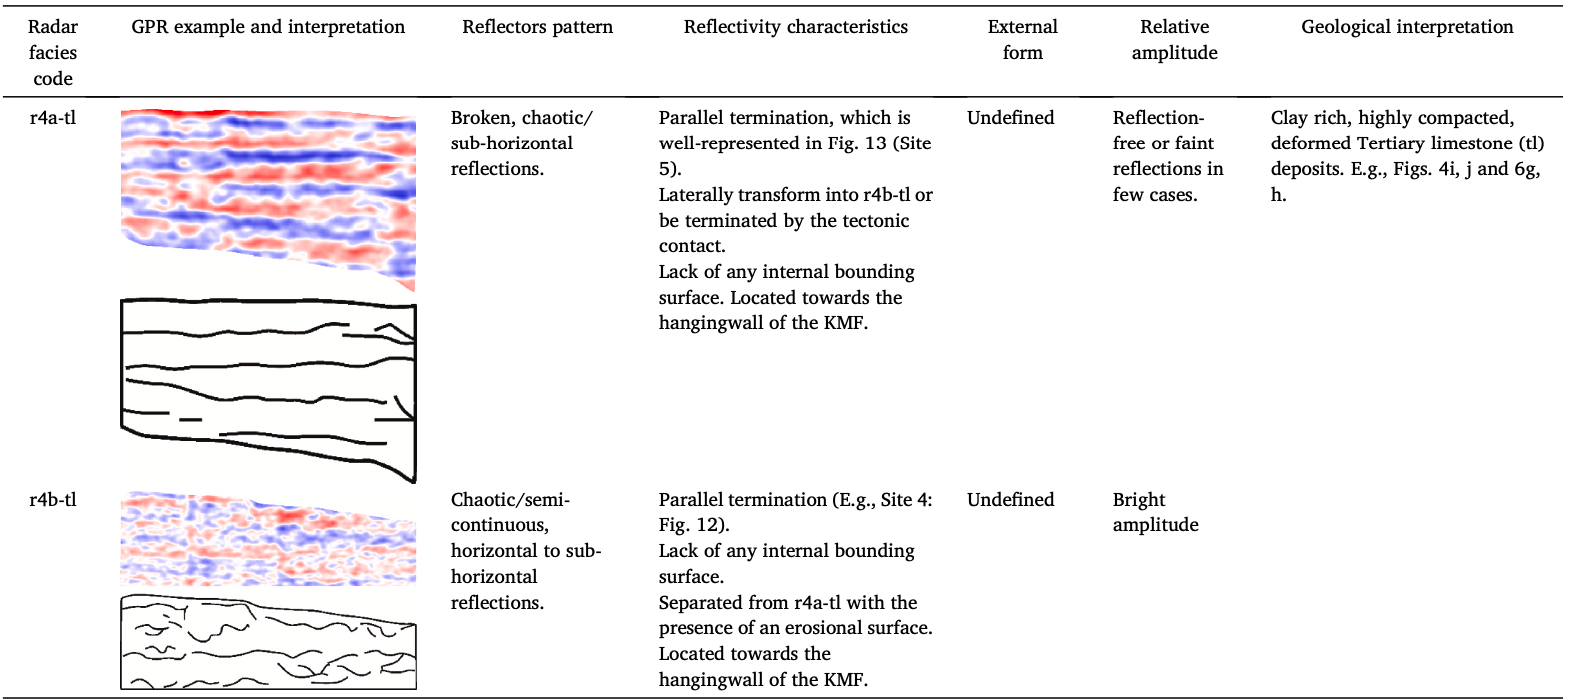
\includegraphics[width=0.9\linewidth]{Figures/0.2GPR/Shaikh2022_fault_2.png}
    \caption[Active fault deposits.]{Active fault deposits. \textbf{Keywords: } Discontinuous, chaotic, sub-horizontal, semi-continuous, horizontal, parallel, high amplitude \citep{Shaikh2022}.}
    \label{fig:Shaikh2022-2}
\end{figure}
\end{landscape}
\clearpage

\begin{figure}[h!]
    \centering
    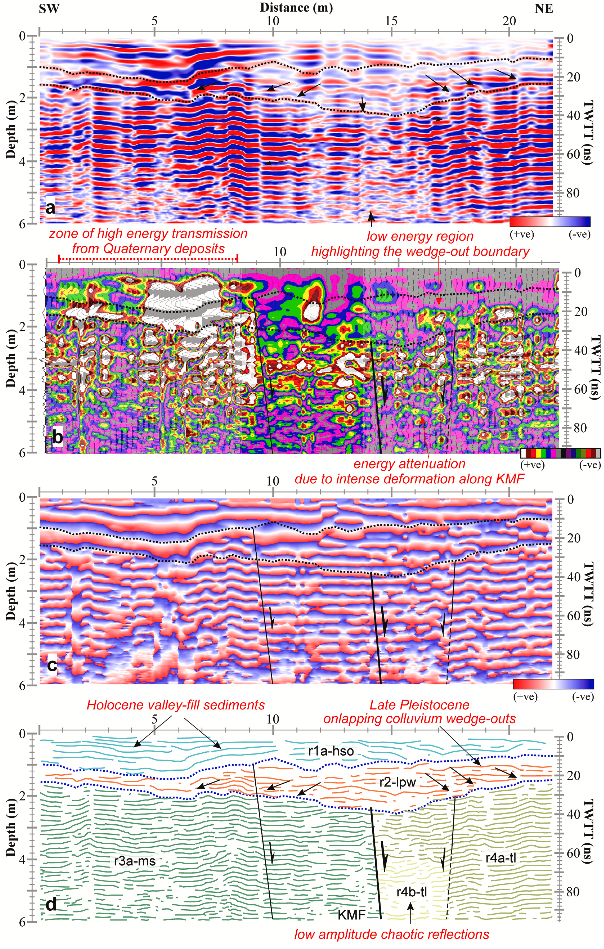
\includegraphics[width=0.9\linewidth]{Figures/0.2GPR/Shaikh2022_fault_3.png}
    \caption[Active fault deposits.]{Active fault deposits. \textbf{Keywords: } Faulting, onlap, high attenuation, discontinuity, continuous \citep{Shaikh2022}.}
    \label{fig:Shaikh2022-3}
\end{figure}
